% Details here
% https://semeval.github.io/paper-requirements.html
\documentclass[11pt]{article}
\usepackage[utf8]{inputenc}
\usepackage[final]{acl}
\usepackage{multirow, makecell}
\usepackage{amsmath}
\usepackage{algorithm}
\usepackage{algpseudocode}
\usepackage{amssymb}
\usepackage{enumitem}
\setlist{nosep, leftmargin=*}
\usepackage{booktabs}
\usepackage{tabularx}
\usepackage{adjustbox}

% Standard package includes
\usepackage{times}
\usepackage{latexsym}
\usepackage{graphicx}
\usepackage{subcaption}
\newcommand\todo[1]{\textcolor{red}{#1}}
\usepackage{xcolor,colortbl}
\usepackage[T1]{fontenc}
\usepackage[utf8]{inputenc}
\usepackage{tcolorbox}
\tcbuselibrary{breakable}
\usepackage{mwe}
\usepackage{tabu}

\usepackage{microtype}

% Compact spacing for professional layout
\setlength{\parskip}{0.3ex plus 0.1ex minus 0.1ex}

% Macros for paper (SemEval-2026 Task 3)
\newcommand{\dimabsaTrainData}{D_{\mathrm{train}}}
\newcommand{\dimabsaTrainActual}{D_{\mathrm{train}}^{80}}
\newcommand{\dimabsaTrainEval}{D_{\mathrm{eval}}^{20}}
\newcommand{\dimabsaTest}{D_{\mathrm{test}}}
\newcommand{\dimabsaDataset}{DimABSA}
\newcommand{\roberta}{XLM-RoBERTa}
\newcommand{\robertaBase}{XLM-RoBERTa\textsubscript{base}}
\newcommand{\model}{base}
\newcommand{\improvement}{$\sim$13\%}
\newcommand{\languages}{\mathcal{L}}
\newcommand{\domains}{\mathcal{D}}



\title{hdharpure at SemEval-2026 Task 3: BERT-Based Modeling and Prediction Behavior Analysis for Multilingual Valence--Arousal Scoring}

\author{
  Harshal Dharpure\textsuperscript{1}, Nicolay Rusnachenko\textsuperscript{2}\\
  \textsuperscript{1} Indian Institute of Technology, Patna \\
  \textsuperscript{2} Centre for Applied Creative Technologies (CFACT+), Bournemouth University, UK  \\
  \texttt{harshal\_2511ai30@iitp.ac.in}, 
  \texttt{nrusnachenko@bournemouth.ac.uk}
} 



\date{January 2024}

\begin{document}

\maketitle


\begin{abstract}
The SemEval-2026 Task 3 is a 
\textit{Dimensional aspect-based sentiment analysis} (DimABSA) task which extends traditional ABSA by predicting continuous regression in two dimensions: valence (V) and arousal (A). 
% Task.
The Track~A/Subtask~1 represent multilingual task in which for a given text and aspects mentioned in it, there is a need to predict V/A scores for each aspect. 
% Methodology.
Our approach is based on the pretraining-finetuning concept: we first pretrain multilingual model ($M'$) followed by its fine-tuning ($M''_{l,d}$) on the training data of specific domain ($d$) and language ($l$).
% Contribution.
We adopt \roberta{} (\model{}) as the encoder with separate regression heads for valence and arousal prediction. 
% Solution.
Our experiments on manual split of official SemEval-2026 Task 3 dataset (\dimabsaTrainEval{}) demonstrate that fine-tuning model in two stages ($M''_{l,d}$) results in average \improvement{} improvement over approach of direct fine-tuning ($M_{l,d}$). 
% Result analysis.
To investigate limitations of the existing approach we visualize and discuss limitations of our system.
% Code.
Our code is publicly available\footnote{\url{https://github.com/harshalDharpure/SemEval-2026-Task-3}}.

\end{abstract}

\section{Introduction}
\label{sec:introduction}

Aspect-based sentiment analysis (ABSA) is a task of predicting sentiment for specific aspects mentioned in text~\cite{liu2012sentiment}. 
\textit{Dimensional} Aspect-Based Sentiment Analysis (DimABSA)~\cite{yu-etal-2026-semeval, lee2026dimabsa} is the task introduced at SemEval-2026 as an extension of traditional ABSA with prediction of continuous scores~\cite{russell1980}. The scores correspond to the following parameters: \textit{valence} and \textit{arousal}. 

\begin{figure*}[!t]
 \centering
  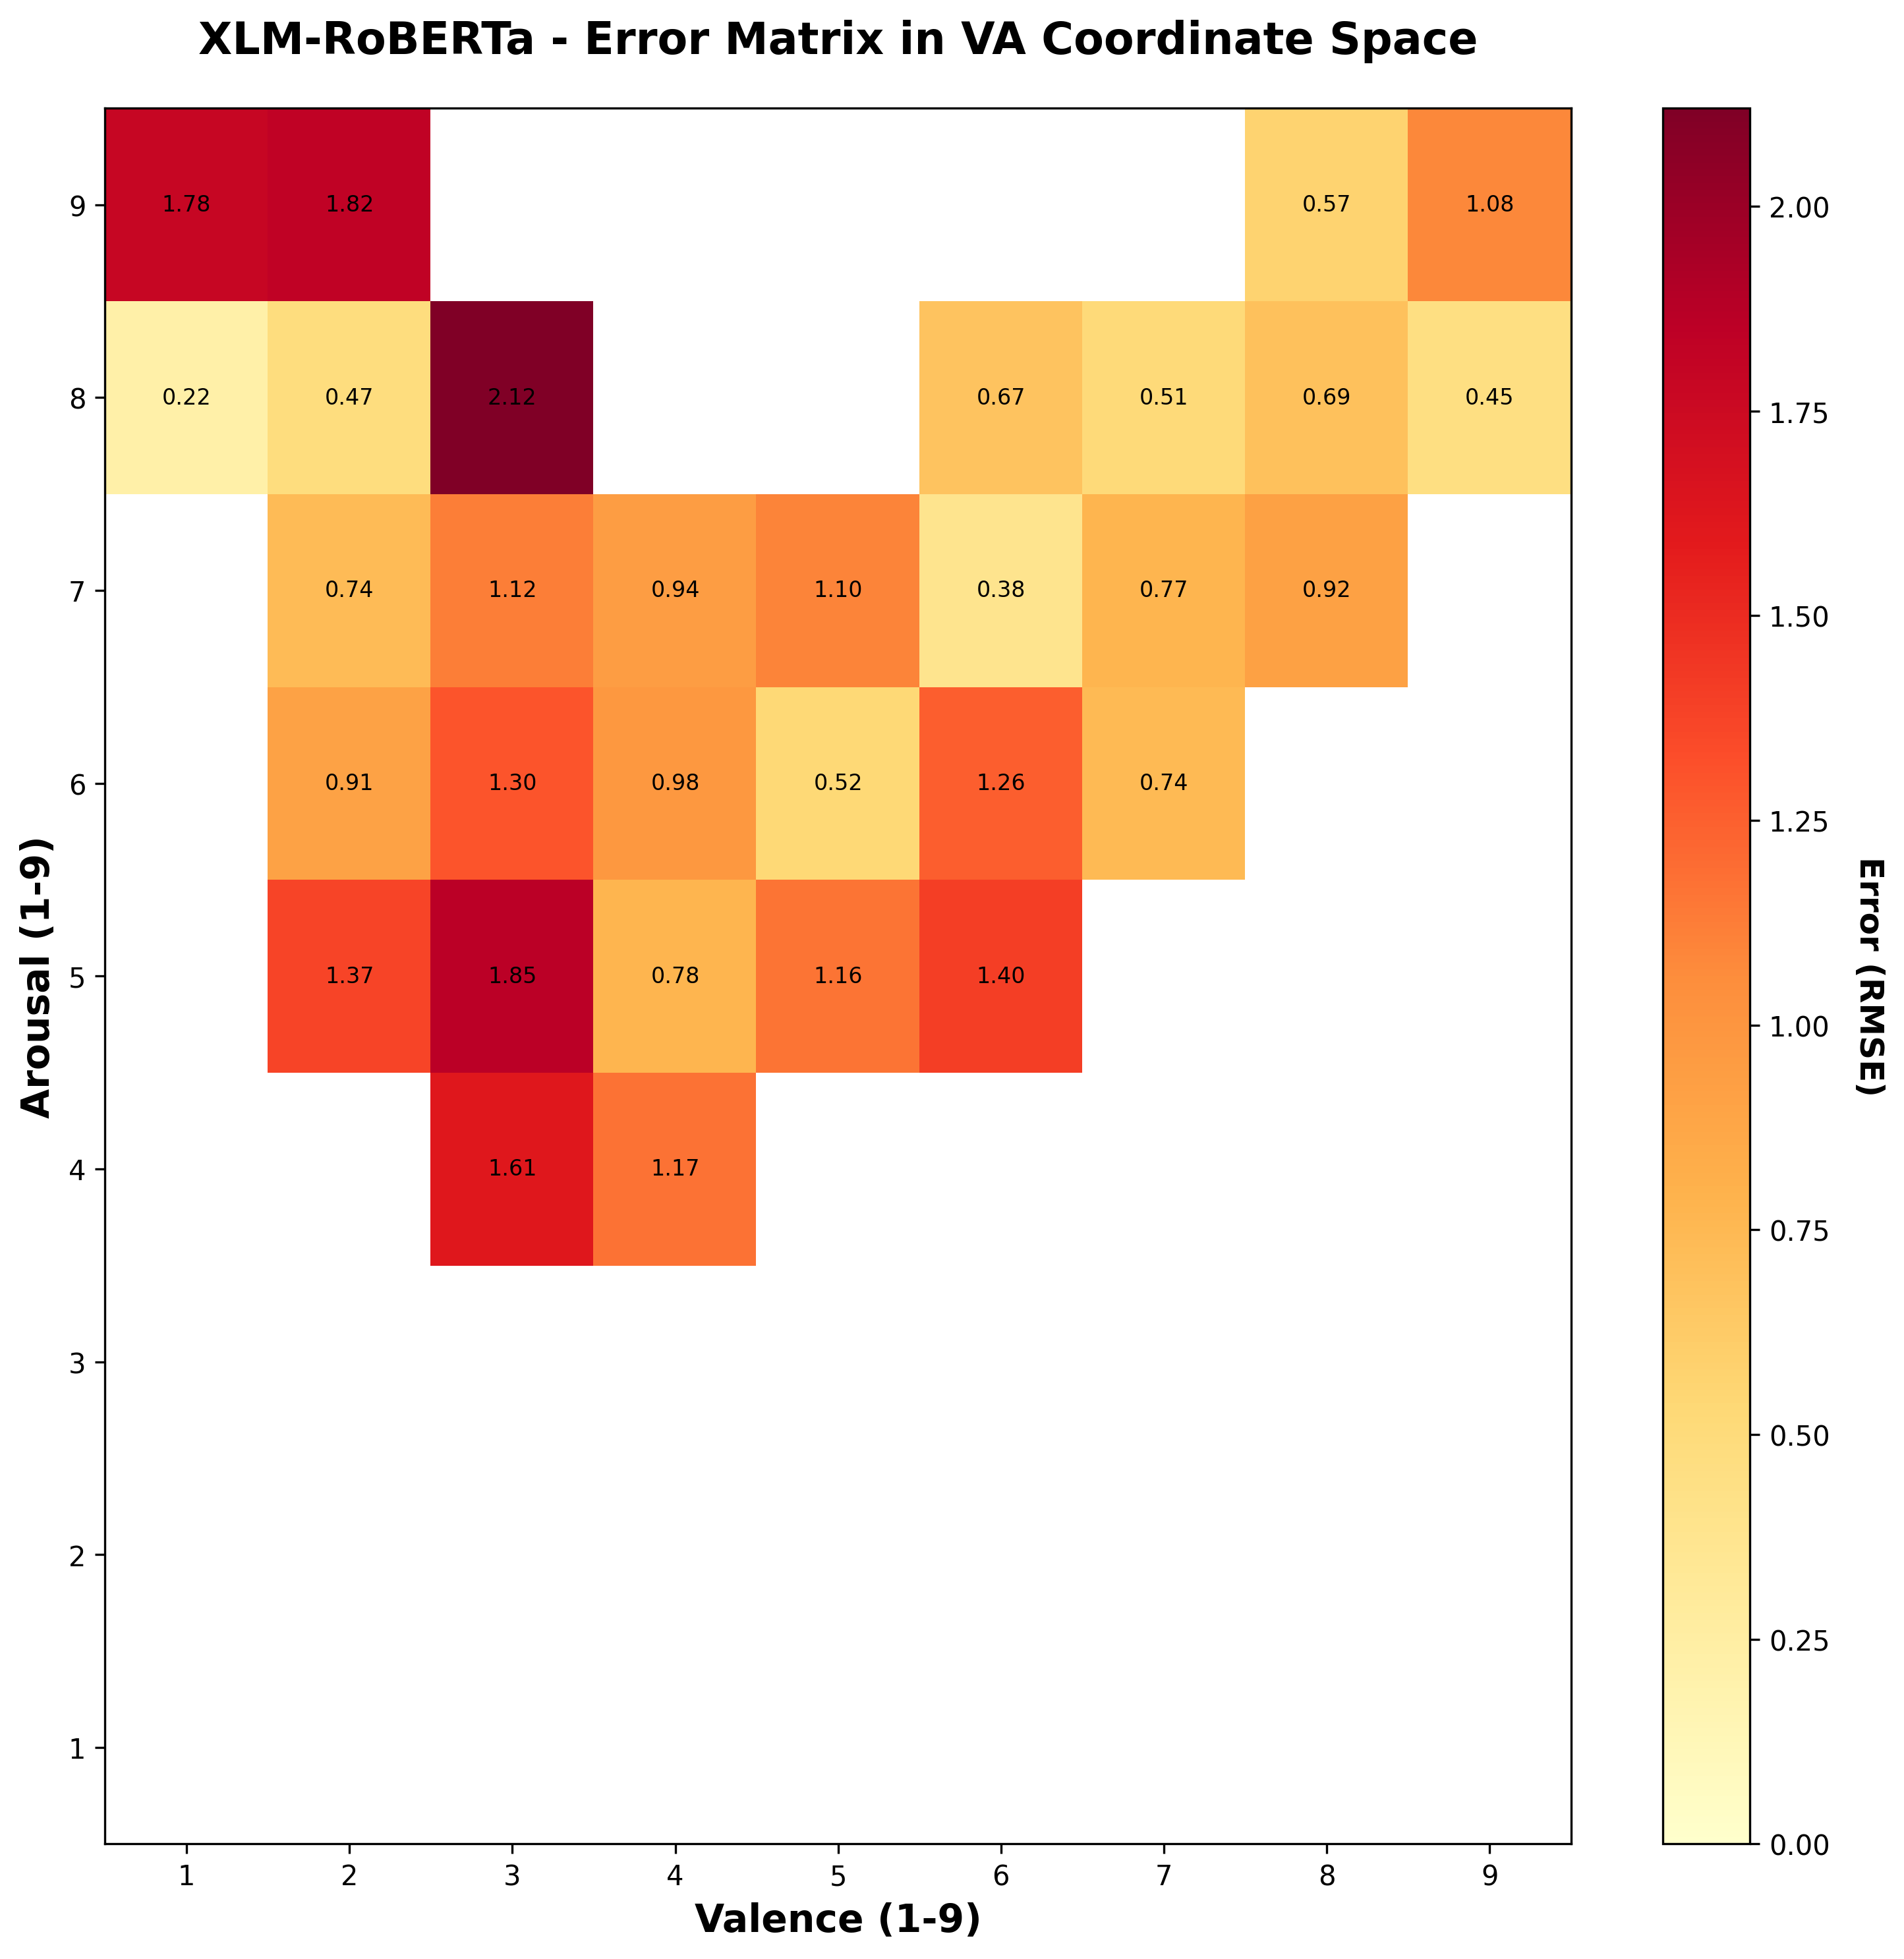
\includegraphics[width=\textwidth]{pics/pipeline.drawio.png}
  \caption{Pretraining-finetuning concept adaptation for model $M$ (left), architecture of the model $M$ (right)}
  \label{fig:pipeline}
\end{figure*}

\textcolor{blue}{[We can find survey to cite here.]}
Due to the specific nature of scores assignation, we believe that using systems that unites language modelling and support regression output represent the best fit with its native adaptation to classification tasks~\cite{rogers-etal-2020-primer}.
The Transformer architecture~\cite{vaswani2017attention} caused a significant impact on the field of Natural Language Processing (NLP), including field of Sentiment analysis. The encoder-based systems, such as BERT~\cite{devlin-etal-2019-bert, liu2019robertarobustlyoptimizedbert} become widely distributed in varios tasks that required classification output.

The DimABSA dataset (\dimabsaDataset{}) and its training part particularly (\dimabsaTrainData{}) shares vast amount of annotated data that unites texts in different languages (English, Japanese, Russian, Ukrainian, Tatar, Chinese) across various domains (Restaurants, Laptop, Finance). 
To leverage the use of cross-lingual and cross-domain data, in this paper we employ \textit{pretraining-finetuning}~\cite{wang2024tutorialpretrainfinetuneparadigmnatural} technique to adapt encoder-based transformers for V/A scoring. We choose \roberta{}~\cite{liu2019robertarobustlyoptimizedbert} for experiments as it is one of the most widely used multilingual transformers.
According to our experiments 
on manually arranged split of training data (\dimabsaTrainEval{}), 
we demonstrate that computing pre-training techniques with further fine-tuning result in \improvement{} improvement.
To study prediction behaviour of the result systems by visualizing alignments in two directions:~(i)~discrepancies of predicted results from reference annotations and (ii)~discrepancies of reference annotations from data distribution in predictions. 
By relying on the observed results on \dimabsaTrainEval{}, we discuss limitations of our approach and suggest further directions to address them.

\section{Methodology}
\label{sec:methodology}

Given $C_{l,d}$ is a collection of texts 
for the particular language $l \in \languages{}$ and domain $d \in \domains{}$. 

\textbf{Task description.} 
For the particular text $t \in C_{l,d}$ with set of aspects mentioned in it $\{\alpha_1, \alpha_2, ..., \alpha_n\}$, 
for each aspect $\alpha_i$, there is a need to predict V/A pair ($v_i', a_i'$) scores.
The $v_i'$ and $a_i'$ are in the range $[1.0, 9.0]$.

Figure~\ref{fig:pipeline}~(left) illustrates the pretraining and fine-tuning concept adaptation for model $M$.
Given model $M$ we compose its domain specific version ($M''_{l_i,d_j}$) by following steps: 
\begin{enumerate}
    \item \textbf{Pre-training}: we unite unite all the collection $C_{l,d}$ for all the languages $l \in \languages{}$ and domains $d \in \domains{}$ into single collection $C$ to compose fine-tuned version ($M'$).
    \item \textbf{Fine-tuning}: for each and particular language $l_i \in \languages{}$ and domain $d_j \in \domains{}$ we use $M'$ to prepare domain specific version ($M''_{l_i,d_j}$).
\end{enumerate}

In our methodology, $M$ is a machine learning model that outputs V/A pair ($v', a'$) scores for a given input context, where $v' \in [0, 9]$ and $a' \in [0, 9]$.
We use Mean Squared Error (MSE) loss for both valence and arousal prediction and compose \textsc{combined loss} (see Figure~\ref{fig:pipeline}) as follows:
\begin{equation}
  \nonumber
  \mathcal{L} = \text{MSE}(v', v) + \text{MSE}(a', a)
\end{equation}
where $v$ and $a$ are ground truth valence and arousal scores, respectively.

Figure~\ref{fig:pipeline}~(right) illustrates the architecture of the model $M$.
We use BERT-based transformer~\cite{liu2019robertarobustlyoptimizedbert}, which supports input for two sentences separated by meta-token (\texttt{[SEP]}) and prefixed by token of class (\texttt{[CLS]}).
For the given text $t$ and particular aspect mentioned in it ($\alpha$) we compose input context as follows:
\begin{align}
    \nonumber
    \texttt{[CLS]}~\alpha~\texttt{[SEP]}~t~\texttt{[SEP]}
\end{align}

To obtain V/A scores we use mean pooling over the sequence, weighted by the attention mask to ignore padding.
The pooled vector is passed through a fully connected layer (FC) with LayerNorm and dropout:
\begin{align}
    \nonumber
    h_{t} &= \text{LayerNorm}(\text{FC}(h_{pooled}))
\end{align}
and then through two heads:
\begin{align}
    \nonumber
    v &= W_v \cdot h_{t} + b_v
    \\
    \nonumber
    a &= W_a \cdot h_{t} + b_a
\end{align}
where $v$ and $a$ are predicted valence and arousal scores in [0, 1] (\textcolor{red}{[Must be in range [1.0, 9.0]]}), and $W_v$ and $W_a$ are weight matrices for valence and arousal, respectively.

\begin{table*}[h]
    \centering
    \footnotesize
    \setlength{\tabcolsep}{2.8pt}
    \renewcommand{\arraystretch}{1.05}
    \begin{tabular}{l|ccc|c|c|cccc|c|cccc}
    \toprule
    \multirow{2}{*}{\textbf{Model}} &
    \multicolumn{3}{c|}{\textbf{eng}} &
    \textbf{rus} &
    \textbf{ukr} &
    \multicolumn{4}{c|}{\textbf{jpn}} &
    \textbf{tat} &
    \multicolumn{4}{c}{\textbf{zho}} \\
    \cline{2-15}
    & Rest. & Laptop & all & Rest. & Rest. & Res. & Hotel & Fin. & all & Rest. & Rest. & Laptop & Fin. & all \\
    \midrule
    \multicolumn{15}{l}{\dimabsaTrainEval{} (Non-official Split)} \\
    \midrule
    Exp1 & 0.81 & 0.87 & 0.84 & 0.84 & 1.01 & -- & 0.48 & 0.61 & 0.54 & 1.29 & 0.47 & 0.61 & 0.33 & 0.47 \\
    Exp2 & 0.88 & 0.78 & 0.83 & 1.01 & 1.07 & -- & 0.46 & 0.59 & 0.52 & 1.25 & 0.47 & 0.61 & 0.47 & 0.51 \\
    Exp3 & \textbf{0.59} & \textbf{0.58} & \textbf{0.58} & \textbf{0.47} & \textbf{0.52} & 0.48 & \textbf{0.39} & \textbf{0.38} & \textbf{0.42} & \textbf{0.92} & \textbf{0.43} & 0.62 & \textbf{0.34} & \textbf{0.46} \\
    \midrule
    \multicolumn{15}{l}{\dimabsaTest{} (Official Split)} \\
    \midrule
    Exp3 & 1.5003 & -- & -- & 1.6515 & 1.7172 & -- & -- & -- & -- & -- & -- & -- & -- & -- \\
    \bottomrule
    \end{tabular}
    \caption{Results (RMSE-AVG $\downarrow$) on \dimabsaTrainEval{} (20\% non-official split) and \dimabsaTest{} (official split) for the XLM-RoBERTa\textsubscript{base} model. Rest.\ = Restaurant. Best per column on TrainEval in bold. Official row: normalized RMSE\textsubscript{VA} (organizers' metric); only eng, rus, ukr submitted.}
    \label{tab:results}
\end{table*}



\input{tables/dataset_stats.tex}

\section{Dataset}
\label{sec:dataset}

The official dataset (DimABSA)~\cite{lee2026dimabsabuildingmultilingualmultidomain,yu-etal-2026-semeval} and available amount of sentences in its training part (\dimabsaTrainData{})  presented in Table~\ref{tab:dataset_stats}.
In this paper we construct splits of the \dimabsaTrainData{} that correspond to: 
\begin{itemize}
    \item \dimabsaTrainActual{} - dataset for pre-training and fine-tuning;
    \item \dimabsaTrainEval{} - dataset for non-official experiments.
\end{itemize}
The splitting is performed at the level of text with inclusion of corresponding aspects mentioned in it. We use random seed (42) to shuffle the texts before splitting.

\subsection{Experimental Setup}

The full model (encoder and regression heads) is trained for 5 epochs with learning rate $1.5 \times 10^{-5}$ with 16 bit float precision. 
For the pre-training we use 5 epochs.
At the Fine-tuning trained with 3 epochs. 
We use \robertaBase{} as the encoder~\cite{liu2019robertarobustlyoptimizedbert} and its initial state further in this section refered as $M$.

\begin{table}[h]
\centering
\small
  \renewcommand{\arraystretch}{1.1}
  \begin{tabular}{@{}ll@{}}
  \toprule
  \textbf{Hyperparameter} & \textbf{Value} \\
  \midrule
  Batch size                & 4 \\
  Max sequence length       & 192 tokens \\
  Learning rate             & $1.5 \times 10^{-5}$ \\
  Dropout                   & 0.1 (encoder), 0.3 (FC layer) \\
  Optimizer                 & AdamW \\
  Mixed precision           & bfloat16 \\
  Early stopping            & Patience 3 epochs (fine-tuning only) \\
  \bottomrule
  \end{tabular}
  \caption{Training configuration}
\label{tab:training_hparams}
\end{table}

For the described methodology in Section~\ref{sec:methodology} we set up the following experiments that involve application of the original model $M$ and its pre-trained version $M'$ pre-trained on the \dimabsaTrainActual{} (see Section~\ref{sec:dataset}).
For the given language $l_i$ and domain $d_j$ we set up the following experiments:
\begin{itemize}
    \item \textbf{Exp1}: Direct fine-tuning $M$ on target language/domain (no pretraining)
    \item \textbf{Exp2}: Inference only $M'$ (no fine-tuning)
    \item \textbf{Exp3}: Fine-tuning $M'$ to obtain $M''_{l_i,d_j}$ used to infer results. 
\end{itemize}

% Result analysis figures (placeholders or include analysis plots)
% Main figures are in pics/ and referenced in the text.
\begin{figure*}[!t]
\centering
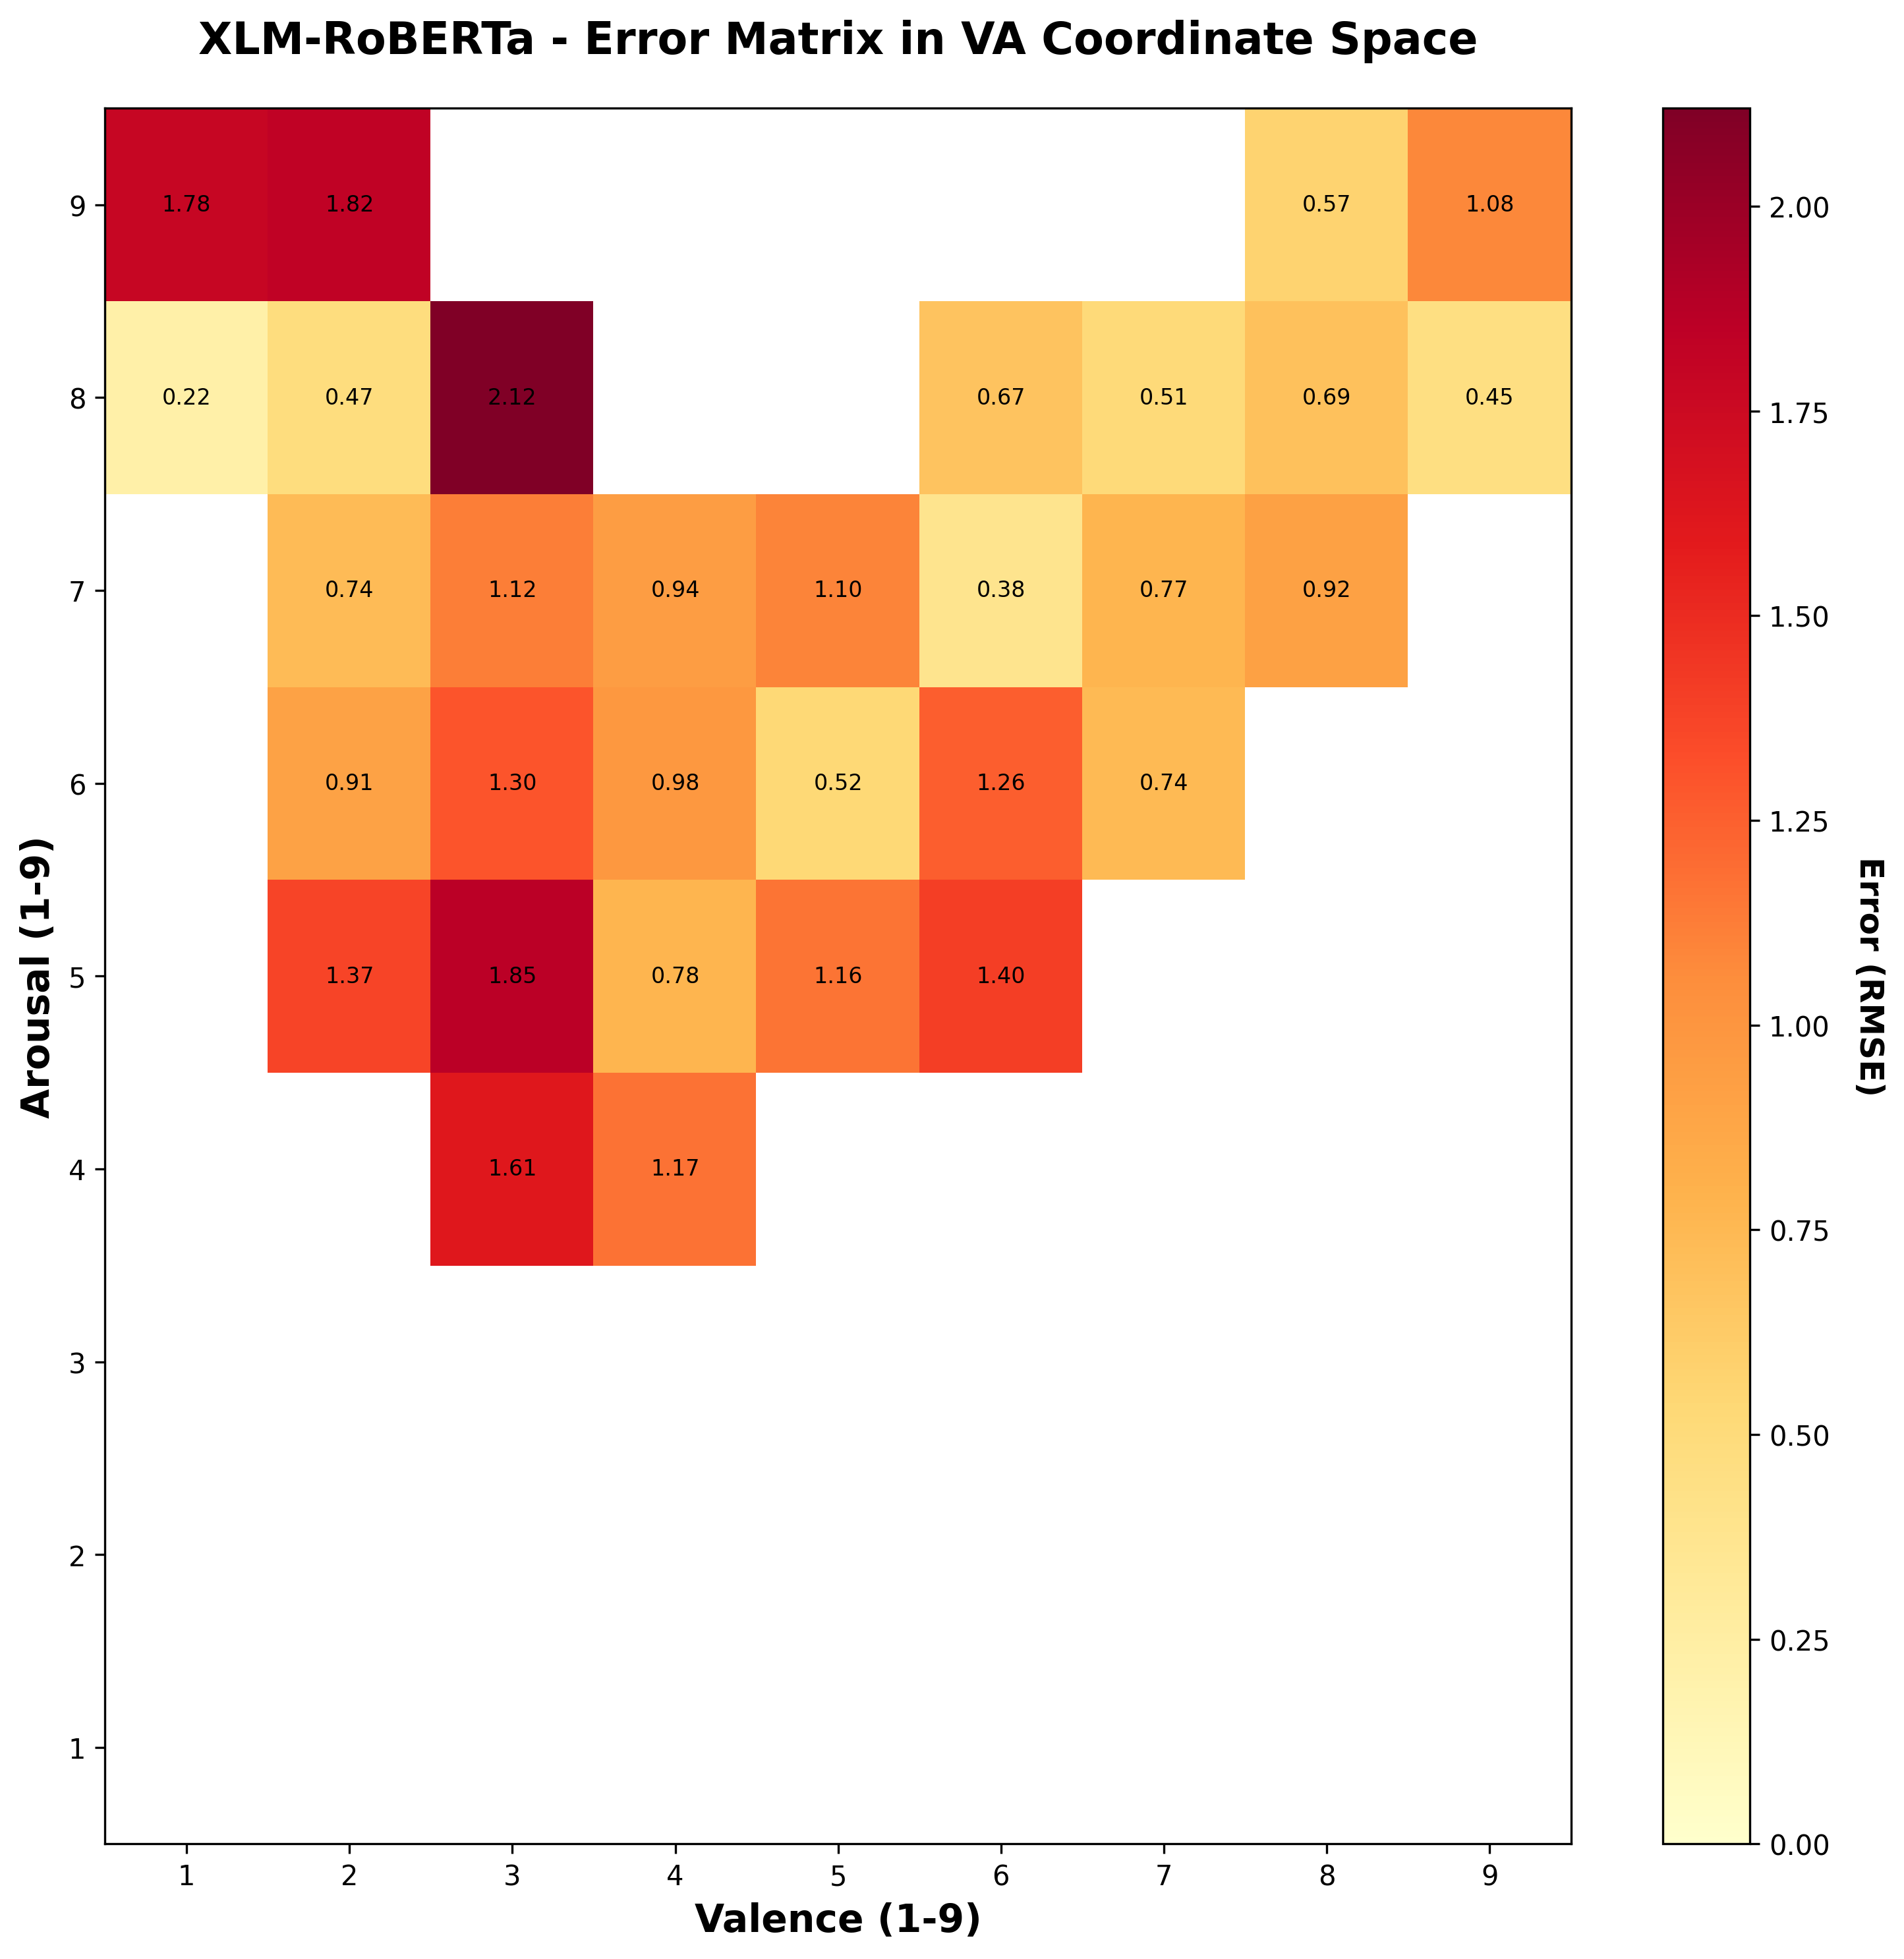
\includegraphics[width=0.48\textwidth]{pics/XLM-RoBERTa_va_space_error_matrix.png}
\hfill
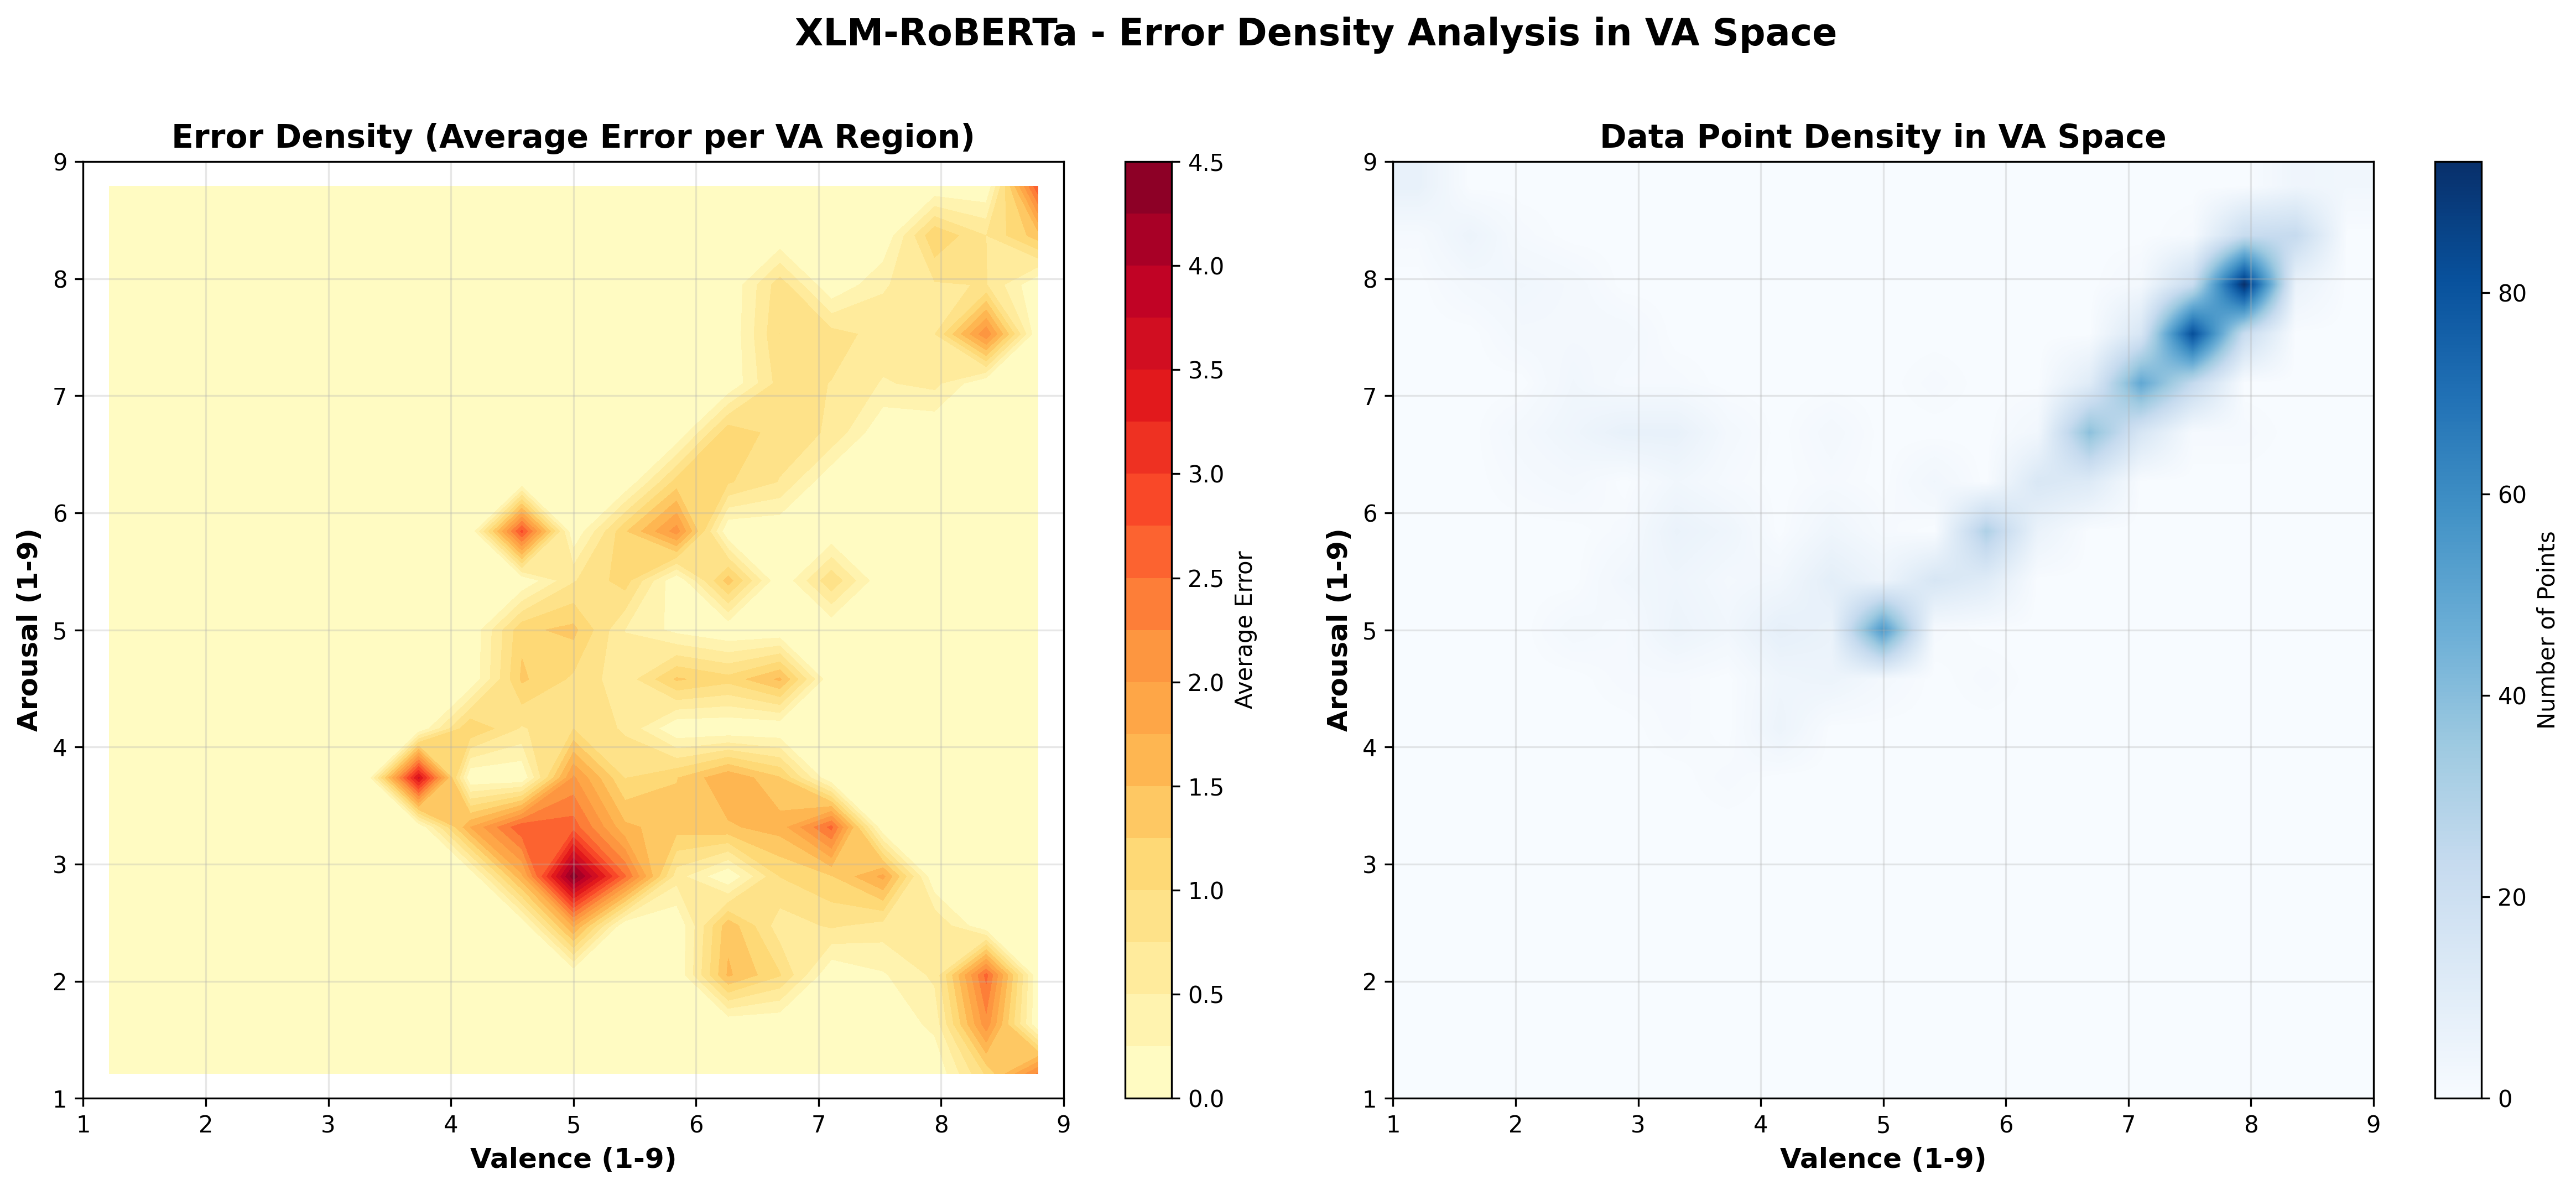
\includegraphics[width=0.48\textwidth]{pics/XLM-RoBERTa_error_density_va_space.png}
\caption{Left: VA space error matrix. Right: Error density in VA space.}
\label{fig:analysis1}
\end{figure*}


For this task, organizers provided the following evaluation metric: RMSE$_{VA}$, which is defined as:
{\small
\begin{equation*}
    \text{RMSE}_{\text{VA}} = \sqrt{\frac{1}{n}\sum_{i=1}^{n} \left[(v_{i}^{'} - v_{i})^2 + (a_{i}^{'} - a_{i})^2\right]}
\end{equation*}
}%
where $n$ corresponds to a total number of pairs $\left<t, \alpha\right>$, and 
$v_{i}$ and $a_{i}$ are ground truth valence and arousal scores, respectively. Lower values indicate better performance.

Table~\ref{tab:results} presents the results for experiments on non-official experiments dataset \dimabsaTrainEval{}, and results of the best performing approach (Exp3) on official test \dimabsaTest{} data.
According to the results observed on \dimabsaTrainEval{}, using adapting pretraining-finetuning concept (Exp3) results in \improvement{} improvement by RMSE\textsubscript{avg} over results in Exp~1.

\textcolor{blue}{[Describe our results on \dimabsaTest{} by outlining our position in leaderboard].}

\section{Result Analysis and Discussion}
\label{sec:result-analysis-and-discussion}

\textcolor{red}{[Setup. restaurant domain (as the most common among all the available data; (languages).; this is eval-20 dataset; this is exp-3 (two-stage); bar pallette varies from 0 to 5.]} \textcolor{red}{[Explain the intention in using hierarchical BERT methods and classifiers.]}
\textcolor{red}{[Gold as reference and misalighments, and then pred as reference.; bins size of 1.0 and 0.25]}

Findings that impact the performance:
\begin{itemize}
    \item Outliers.
    \item Out-of-bounds (prediction space could be cropped)
    \item Our model is weak to capture the interdependency in the central area.
Square box 4-6 VA, see [Rus, tatar, URK]
\end{itemize}

Adopt NLI to use output from \texttt{[CLS]} token in area classification~\cite{sun2019utilizing} for the purpose of artificially augmenting the training data. One example we believe: chunking space into areas 
if we re-center the space and give lexical definitions to VA areas.



\section{Conclusion}
\label{sec:conclusion}

This paper presents a study on adapting encoder-based transformers in novel task, dubbed as dimentional aspect-based sentiment analysis (DimABSA) presented as SemEval-2026 as Task~3.
This task extends tranditional ABSA with prediction of continuous scores for valence and arousal.
DimABSA has a multilingual and multidomain setup, and to leverage the use of cross-lingual and cross-domain data, we this paper contribute by investigating effect of pre-training on the model performance.
According to our experiments that involve application of \robertaBase{} model, we demonstrate that pretraining-finetuning concept results in \improvement{} improvement over direct domain and language specific fine-tuning.
We analyse the result of the best performing approach and provide insights about the limitations with further directions to addressing them.


\bibliography{main}

\end{document}